\documentclass[twocolumn, 12pt]{IEEEtran}

\usepackage[margin=0.5in]{geometry}

\usepackage{amsfonts,amsmath,amssymb,amsthm,bm,relsize,textcomp}
\usepackage{balance}
\usepackage{graphicx}
\usepackage[bottom]{footmisc}

\begin{document}

\title{Project Assignment 2: Report}
\author{Johannes Lemonde 960911-T357 and Lucas Streit 970606-T???}
mettre le numéro personnel de Lucas

\maketitle

\section{Introduction}

The main concern of this project is to decode a signal which was distorted by an unknown time-invariant finite impulse response filter and which includes also some white noise. Such filters are commonly used by communication channels; our role here is to take a glimpse into the maths behind the receptor -- in other words, to elaborate the algorithm able to decode this distorted signal back to the original signal.

We are provided with such a distorted signal consisting of a large sequence of real numbers, knowing that the original binary signal --~before it was distorted~-- starts with a given binary sequence, which we also know.

The knowledge of this sequence at the beginning of the signal is needed by the receptor to compute a set of constant parameters, comparing the original and distorted signals --~through a system of linear equations to solve~--, which would then be used to determine the further bits of the original signal.

To make this project fancier, we are dived into a situation where the original signal is a key to decipher a picture. We are given an encrypted picture and the ciphering/deciphering algorithms, and the better the recovered key, the more accurate the deciphered picture.

\section{Formalisation of the problem}

 The original binary signal -- the key -- is composed by a sequence ${b(k)\in \{-1,1\}}, ~~{k\in[1, M]\subset\mathbb{N}}$, where $M$ is the length of the key.\footnote{Actually, the key is originally composed by a sequence ${s(k)\in\{0,1\}}$, but we map it with the sequence ${b(k)\in\{-1, 1\}}$.}
 The values ${b(1),~\dots~, b(N)}$ --~referred to as the training sequence~-- are known to us, with ${N=32}$.
 Before it was transmitted, the key has been subjected to an unknown filter $h$ of order ${3}$ and to the white noise $n(k)$ such as 
 \begin{equation}\label{eq:r}
 { r(k) = \sum\limits_{l=0}^{3}h(l)~b(k-l)~+n(k),~~k\in[1,M]\subset\mathbb{N} }.
 \end{equation}
 These values of $r$ are known to us, and we are asked to reconstruct the sequence $b$.
 
 \section{Resolution}
 
 In order to do so, we apply an equaliser (an other filter) of order $L$ such as 
 \begin{equation}\label{eq:bt}
 { \hat{b}_{r}(k) = \sum\limits_{l=0}^{L}w(l)~r(k-l) \approx b(k) },
 \end{equation}
 where the coefficients ${w(0)},~{\dots~},{w(L+1)}$ must be initialised using the training sequence. To do so, we define a matrix $\bm{R}$, a vector $\bm{w}$ and a vector $\bm{b}$ so that $\bm{Rw}=\bm{b}$ represent the equations in (\ref{eq:bt}). Since $r(k)$ does not have values for $k$ being null or negative, and since we have this subtraction of $l$ in the argument of $r$ in (\ref{eq:bt}), we can only use (\ref{eq:bt}) for $k = L+1,~\dots~, N$, which thus gives $\bm{Rw}=\bm{b} \Leftrightarrow $
\begin{equation}\label{eq:matrixes}
\begin{pmatrix}
    \mathsmaller{r(L+1)}   & \mathsmaller{r(L)} & \mathsmaller{\cdots}  & \mathsmaller{r(1)} \\
    \mathsmaller{r(L+2)}   & \mathsmaller{r(L+1)} & \mathsmaller{\cdots}  & \mathsmaller{r(2)} \\
    \mathsmaller{\vdots}   & \mathsmaller{\vdots} & \mathsmaller{\cdots} & \mathsmaller{\vdots} \\
    \mathsmaller{r(k)}     & \mathsmaller{r(k+1)} & \mathsmaller{\cdots} & \mathsmaller{r(k-L)} \\
    \mathsmaller{\vdots}   & \mathsmaller{\vdots} & \mathsmaller{\cdots} & \mathsmaller{\vdots} \\
    \mathsmaller{r(N)} & \mathsmaller{r(N-1)} & \mathsmaller{\cdots}  & \mathsmaller{r(N-L)}
%   a & b
\end{pmatrix}
\cdot
\begin{pmatrix}
   \mathsmaller{w(0)}\\
   \mathsmaller{w(1)}\\
   \mathsmaller{\vdots}\\
   \mathsmaller{w(L)}
\end{pmatrix}
=
\begin{pmatrix}
   \mathsmaller{b(L+1)}\\
   \mathsmaller{b(L+2)}\\
   \mathsmaller{\vdots}\\
   \mathsmaller{b(k)}\\
   \mathsmaller{\vdots}\\
   \mathsmaller{b(N)}
\end{pmatrix}
\end{equation}

Notice that $\bm{R}$ is not square for any value of $L$, so the system might have much more equations than unknowns. Thus, resolving the system for $\bm{w}$ results in resolving it in the approximation of the least squares: $\bm{w} \approx (\bm{R}^{T}\bm{R})^{-1}\bm{R}^{T}~\bm{b}$. Matlab does this automatically for non-square matrices with the command \texttt{w~=~R\textbackslash b}.

Once these coefficients $\bm{w}$ are computed, we can freely use the equation (\ref{eq:bt}) to get the estimated values $\hat{b}_{r}(k)$ of the whole signal (for $k \leq N$, and especially for $k \leq L$, we use the known training sequence directly, instead), but we still need to convert them to a binary sequence. In order to do so, we apply a sign detector on the real-valued estimator of $b$, which gives: $\hat{b}(k) = sign(\hat{b}_{r}(k)) = \{_{-1,~\hat{b}_{r}(k) \leq 0}^{+1,~\hat{b}_{r}(k) > 0}$.

\section{Optimisation of the equaliser's order $L$}
We have now everything needed to reconstruct the key, apart from $L$. Indeed, the accuracy of the recovery of the key depends on the choice made for the order of the equaliser.

On the first hand, having a really low order $L$ for the equaliser would be insufficient to cancel out the white noise (see figure \ref{fig:f2}). Indeed, the expected value of the white noise tends towards zero if we consider a great amount of its realisations, so increasing $L$ would result in a better cancellation of the noise. Whereas the effects of the unknown filter $h$ in (\ref{eq:r}) are much easier to restore, even with a quite low order equaliser.

\begin{figure}[h]
   \begin{center}
      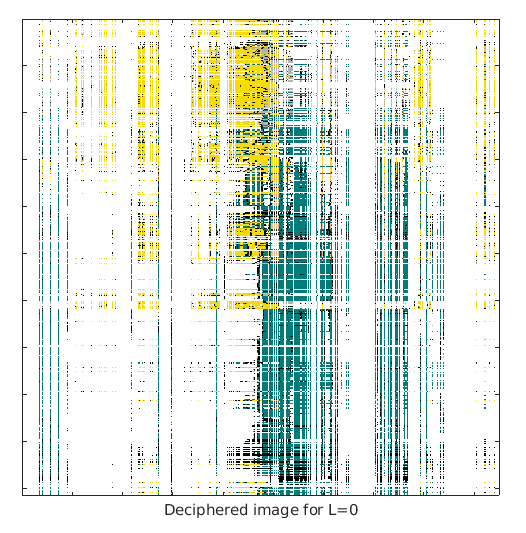
\includegraphics[width=.33\linewidth]{l0.png} \nolinebreak 
      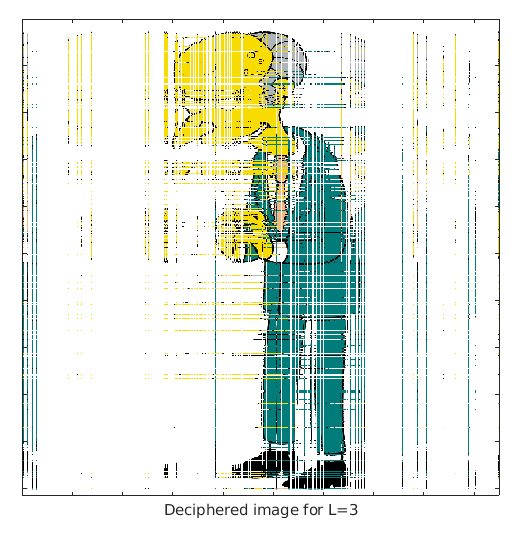
\includegraphics[width=.33\linewidth]{l3.png} \nolinebreak 
      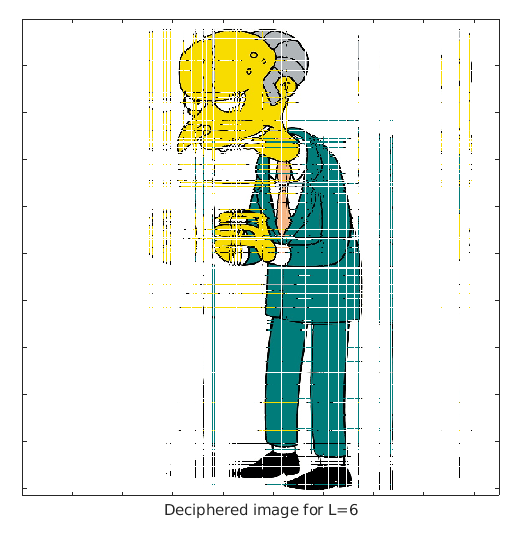
\includegraphics[width=.33\linewidth]{l6.png}
   \end{center}
\vspace{-0.6cm}
\caption{The deciphered image shows \textit{Mr. Burns}, a character out of the American animated sitcom \textit{The Simpsons}. Here, it was deciphered with an equaliser order $L$ of respectively $0$ (no equaliser), $3$ and $6$.}
\label{fig:f2}
\end{figure}

On the other hand, increasing the order $L$ results in decreasing the amount of linear equations and thus the amount of values of the training sequence we are going to be able to use. Indeed, the amount of equations is equal to $N-L$ while the amount of unknowns is $L+1$. 

For a great order $L > \frac{N-1}{2} = 15.5$, the system of equations is under-determined and this results in very few values $b(k)$ determining a large amount of coefficients $w(k)$ as if one tried to project a vector into a greater dimension as its own: an infinity of solutions exist. Even if the training sequence $b(k)$ for ${k=L+1,~\dots~, N}$ can be recovered perfectly with $\hat{b}_{r}(k)$, the extrapolation on further values of the key does not work. In this case, the key contains to many errors to decipher the image accurately (see third image in figure \ref{fig:f1}).

%ERROR-ERROR-ERROR-ERROR-For $L=\frac{1}{2}(N-1)$, if $N$ was odd, the matrix $\bm{R}$ would be square and there would be exactly one solution to the system of linear equations -- under the assumption that no equation is a linear combination of other equations. 

For $L < \frac{N-1}{2} = 15.5$, the system of equations is over-determined and its solution is in the sense of the least-squares. Considering the fact that the equations around the training sequence are not necessarily perfectly representative of the following of the key, due for example to aberrant noise values misleading the calculation of the coefficients $w(k)$, it seems to be an advantage to have (some) degrees of over-determination.

Empirically, the accuracy of the key recovery is the best for $L=12$ or $L=13$, quite good for ${L \in [7,14] \subset \mathbb{N}}$, while the image is only just recognisable for $L=15$.

\begin{figure}[h]
   \begin{center}
      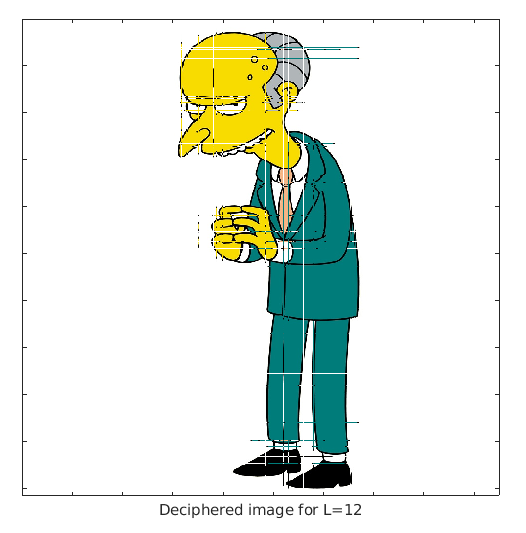
\includegraphics[width=.33\linewidth]{l12.png} \nolinebreak 
      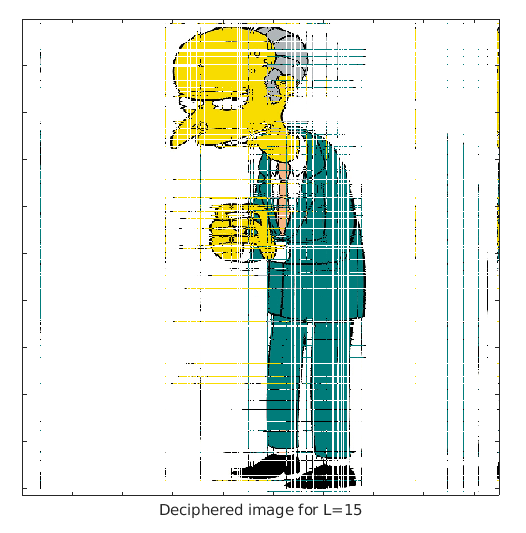
\includegraphics[width=.33\linewidth]{l15.png} \nolinebreak 
      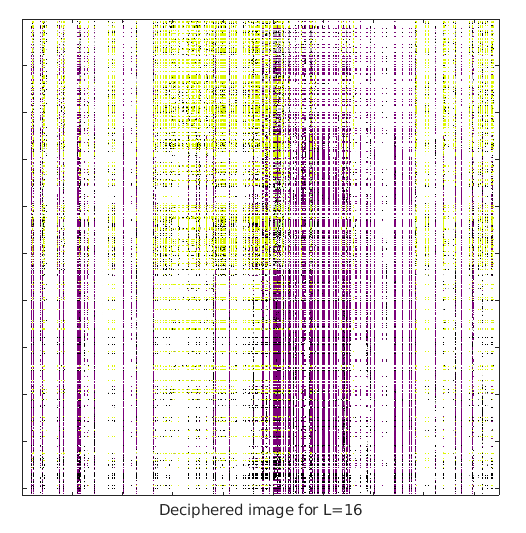
\includegraphics[width=.33\linewidth]{l16.png}
   \end{center}
\vspace{-0.6cm}
\caption{Here, the image was deciphered with an equaliser order $L$ of respectively $12$, $15$ and $16$.}
\label{fig:f1}
\end{figure}

While trying to generate a new sequence $r(k)$ according to the equation (\ref{eq:r}), using to do so an arbitrary original key $b(k)$, a filter set arbitrarily to 
$$
h(l) =
\left\{
	\begin{array}{ll}
		1  & \mbox{if } l = 0, \\
		0.7 & \mbox{if } l \in \{1, 2, 3\}, \\
		0 & \mbox{else.}
	\end{array}
\right.
$$
and white noise $n(k) \stackrel{\text{i.i.d.}}{\sim } \mathcal{N}(0, 0.2^2)$, we obtain for the mean square error ${MSE = \frac{1}{M}\sum\limits_{k=1}^{M}(\hat{b}(k)-b(k))^2}$ in function of the equaliser's order $L$ the graph shown in figure \ref{fig:g}, which seems to confirm our suspicions.
\begin{figure}[h]
   \begin{center}
      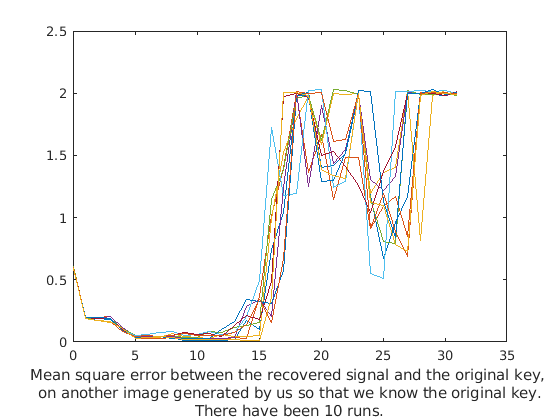
\includegraphics[width=.8\linewidth]{tse4.png}
   \end{center}
\vspace{-0.6cm}
\caption{The MSE increases drastically from the point where the system is under-determined ($L\geq 16$).}
\label{fig:g}
\end{figure}
Obviously, we do not have at our disposal the actual function $h$, nor the actual realisations of the Gaussian white noise, nor even its variance, and according to the many invocations of randomness during the generation of the key (random ciphering of the image) and the noise, the shape of this graph does change a lot from an execution to another. However, the amount of errors seems to be always drastically higher for $L > \frac{N-1}{2}$, while is remains low for an order $L$ between $1$ and $15$, especially in the upper middle of this range.



\section{Random bit error insertions}

In this section of the report, we are going to discuss the impact of the insertion of bit errors upon the quality of the image recovery. In the general case, this depends much on the algorithm in use to cipher/decipher the image as some algorithms could make it very hard to recover anything from the fist bit error.

\begin{figure}[h]
   \begin{center}
      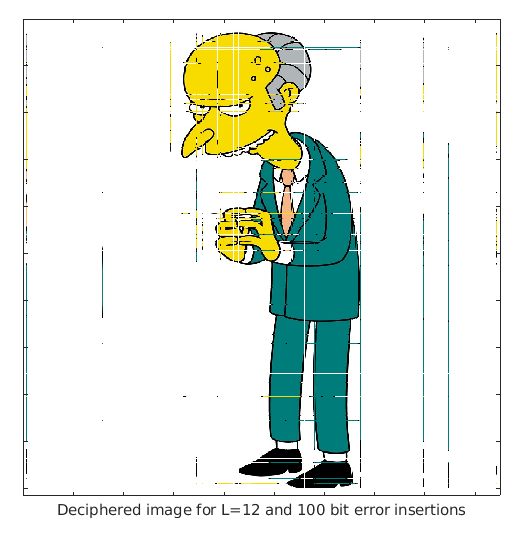
\includegraphics[width=.33\linewidth]{l12e2.png} \nolinebreak 
      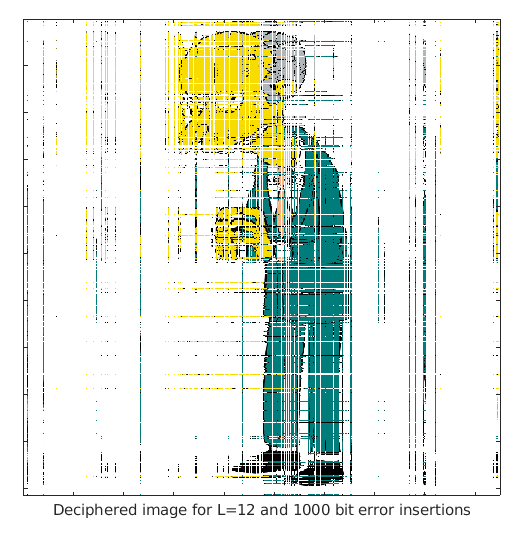
\includegraphics[width=.33\linewidth]{l12e3.png} \nolinebreak 
      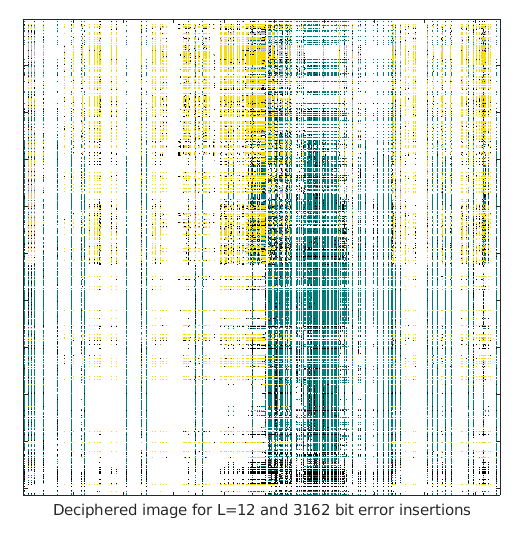
\includegraphics[width=.33\linewidth]{l12e3-5.png}
   \end{center}
\vspace{-0.6cm}
\caption{Here, the image was deciphered with an equaliser order $L=12$ and $10^2$, $10^3$ and $10^{3.5}$ bit errors were inserted, respectively.}
\label{fig:e}
\end{figure}

Nevertheless, in this specific case, the algorithm seems to traduce \textit{linearly} the amount of inserted bit errors as amount of permutations of lines, rows or colours of pixels.\footnote{Images are seen here as a tridimensional matrix where the third dimension is the intensity of red, green and blue of the pixels. The ciphering/deciphering algorithm swaps basically plans within the matrix representing the image. Since the third dimension is only made by three plans while the other two dimensions are made up by as many plans as the image's amount of row or columns, and since the algorithm seems to pick uniformly which permutation it is about to perform, the probability to swap colours is quite low. Here, the matrix' dimensions are 1015x950x3.}

Using this, we can visually suppose that our performance recovering the key with $L=12$ gave about $10^2$ bit errors, and with $L=15$ it was less than $10^3$ errors, for a key length of ${19712}$; in other words, respectively about $0.5\%$ and less than $5\%$.

Moreover, we find that the limit to recognise the subject of the image lies around these $10^{3}$ bit errors, corresponding to $5\%$. 


\section{Conclusion}

With this project, we have been able to understand the basic functioning of some kind of communication channels and have taken a closer look at channel distortion through a finite impulse response filter as well as linear equalisers. Since this equaliser was linear -- rather than optimal -- it was as expected not possible to recover the key perfectly. But it was still possible to get quite a good result so it was achievable to recognise the subject on the deciphered picture.



\begin{thebibliography}{1}

\bibitem{HanOttHjalm}
P. Handel, R. Ottoson, H. Hjalmarsson, \emph{Signal Theory}, KTH, 2012

\end{thebibliography}

\balance

\end{document}
